

\chapter{再評価手法の有効性の確認のための歩行シミュレーション}\label{chapter:再評価手法の有効性の確認のための歩行シミュレーション}
第\ref{chapter:再評価手法の有効性の確認のための歩行シミュレーション}章では,
実装した再評価手法の有効性を確認するために,シミュレーションを用いた歩行実験を行い,その結果を示す.

\section{直進動作の自由歩容パターン生成シミュレーション}
まずは,直進動作の自由歩容パターン生成シミュレーションを行い,再評価手法の有効性を確認する.

\subsection{シミュレーション実験の目的}
シミュレーション実験の目的は,
再評価手法によって生成された自由歩容パターンを用いて,
脚軌道生成の失敗が生じないことを確認することとする.

波東らの研究で実機では歩行することができなかった地形を含む5種類の地形を歩行させ,
脚軌道生成の失敗の回数が0回となることを確認する.
また再評価手法の利点として,計算時間が大幅に伸びないことが期待されるため,計算にかかる時間も測定する.

\subsection{シミュレーション実験の条件}
シミュレーションには,\chref{chapter:歩容パターンの再評価手法の提案}で使用したシミュレーションソフトウェアを使用した.
また,計算環境も同じく\tableref{tab:simulation_env}に示したものを用いており,
シミュレーションのモデルとしたロボットも同じくPhantomXとした.

\subsubsection{歩行する地形}
シミュレーションに使用する地形を\figref{fig:ch5_simu_terrain}に示す.
また矢印でロボットの進行方向を示した.
シミュレーションに使用した地形は,平面,130mmの上り段差,130mmの下り段差,15度の上り斜面,15度の下り斜面の5種類である.
\chref{chapter:歩容パターンの再評価手法の提案}で行ったシミュレーションの条件から変更し,上り段差と下り段差の高さを130mmとしている.

\subsubsection{歩行する時の条件}
シミュレーション時の歩行条件は以下の通りである.
\begin{itemize}
  \item 胴体姿勢は常に水平である.
  \item 最小半径を$130 [mm]$とし,再評価時には最小半径を$140 [mm]$に変更する.
  \item 重心から見た遊脚高さを$-20 [mm]$とする.
  \item 胴体を地形から最小$30 [mm]$離す.
  \item 常に静的安定余裕は$15 [mm]$以上を保つ.
\end{itemize}
最小半径を\figref{fig:ch5_range_revaluation}に示す.
この図は\figref{fig:simu_leg_range}と同様に,横軸をx軸,縦軸をz軸としており,単位は$[mm]$である.
実際の可動範囲を黒の線で示し,近似された可動範囲を緑の線で示している.
また,再評価時の近似された可動範囲を黄緑の線で示しており,遊脚高さを赤い線で示している.

\begin{figure}[htbp]
  \centering
  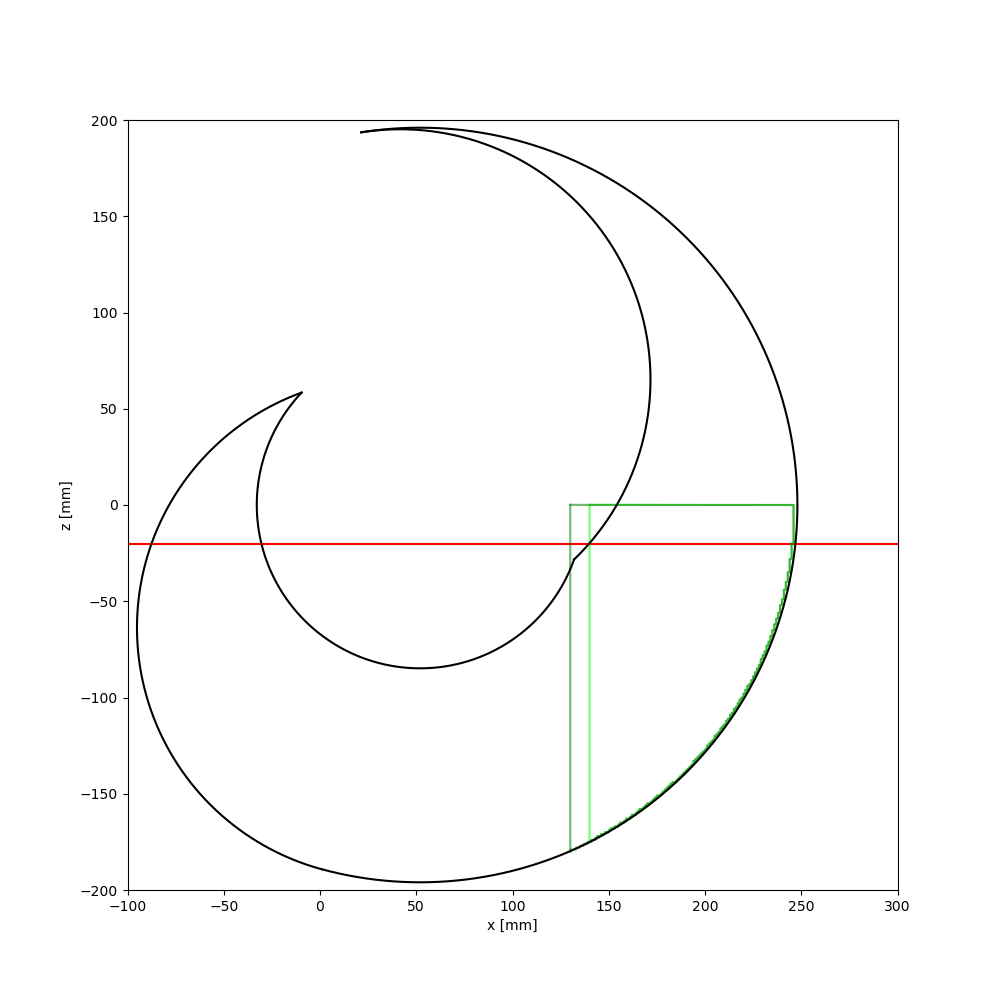
\includegraphics[width=0.5\linewidth]{figure/chapter4/revaluation_view.png}
  \caption{Leg Range of Motion for Revaluation Method}
  \label{fig:ch5_range_revaluation} % chktex 24
\end{figure}

\subsubsection{シミュレーションの手順}
各地形で水平方向に$1200 [mm]$直進するまでの自由歩容パターンを生成した.
\figref{fig:ch5_simu_terrain}のロボットの初期位置をランダムに変化させて計5回ずつ歩行させた.
再評価手法を用いた場合と用いていない場合を比較するため,
再評価手法を用いず初めから最小半径を$140 [mm]$としたプログラムを用いて同様のシミュレーションを行った.
シミュレーションごとに,脚軌道生成の失敗の回数,脚先座標,計算時間を測定した.


% 地形の図
\begin{figure}[htbp]
  \begin{tabular}{cc}
    \begin{minipage}[t]{0.45\hsize}
      \begin{center}
      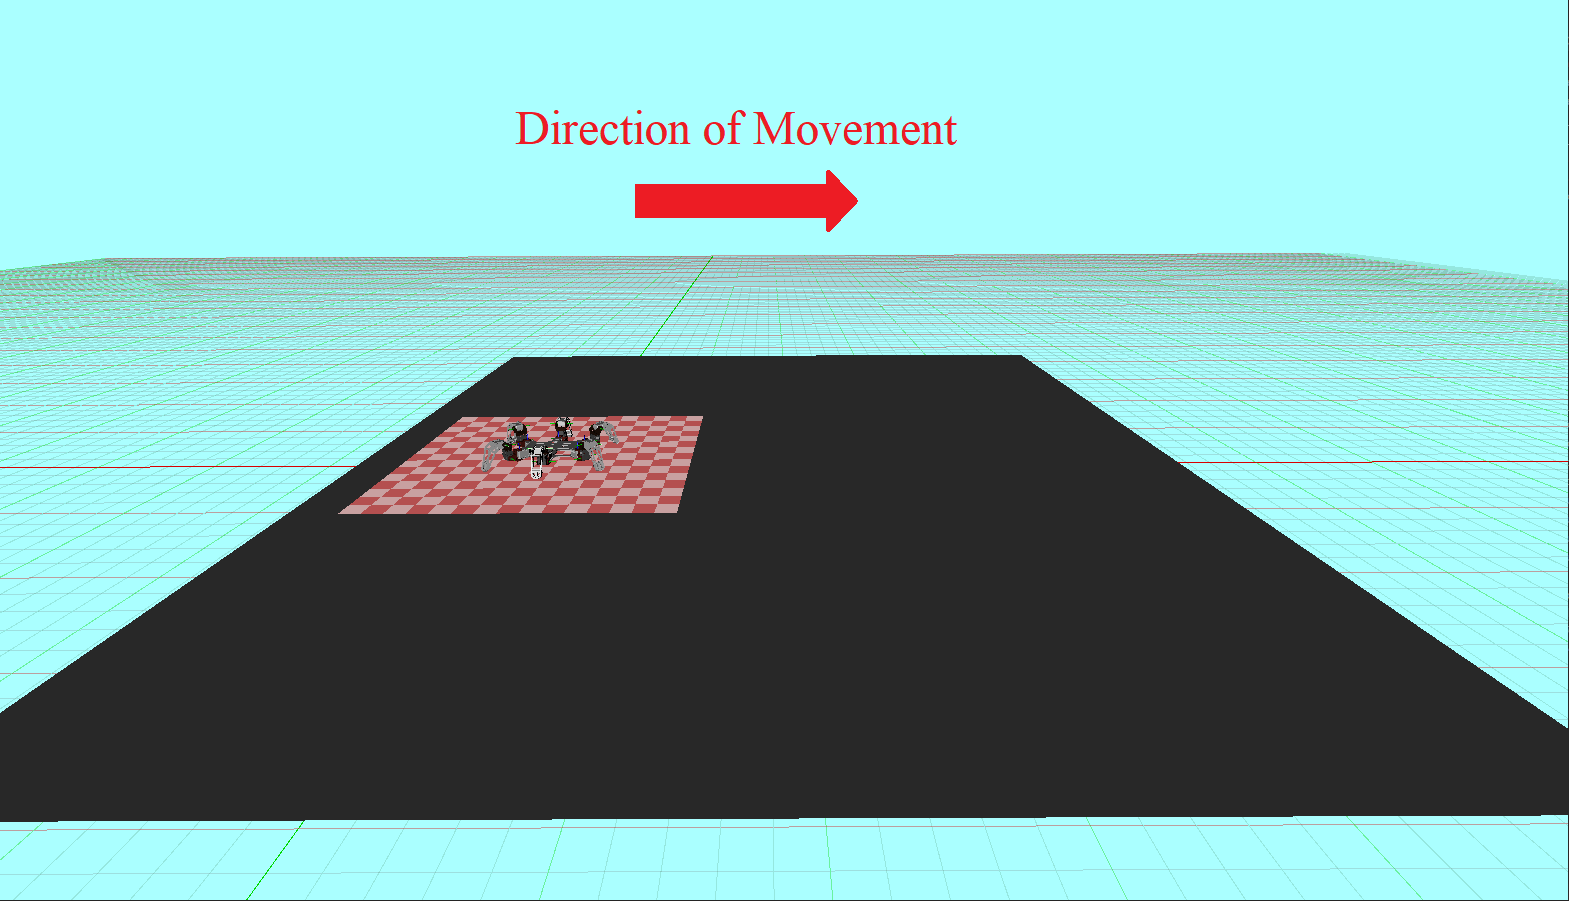
\includegraphics[width=1.0\linewidth]{figure/chapter4/map_flat.png}
      \text{(a) flat}
      \label{fig:ch5_simu_terrain_flat} % chktex 24
      \end{center}
    \end{minipage} 
    &
    \begin{minipage}[t]{0.45\hsize}
      \begin{center}
      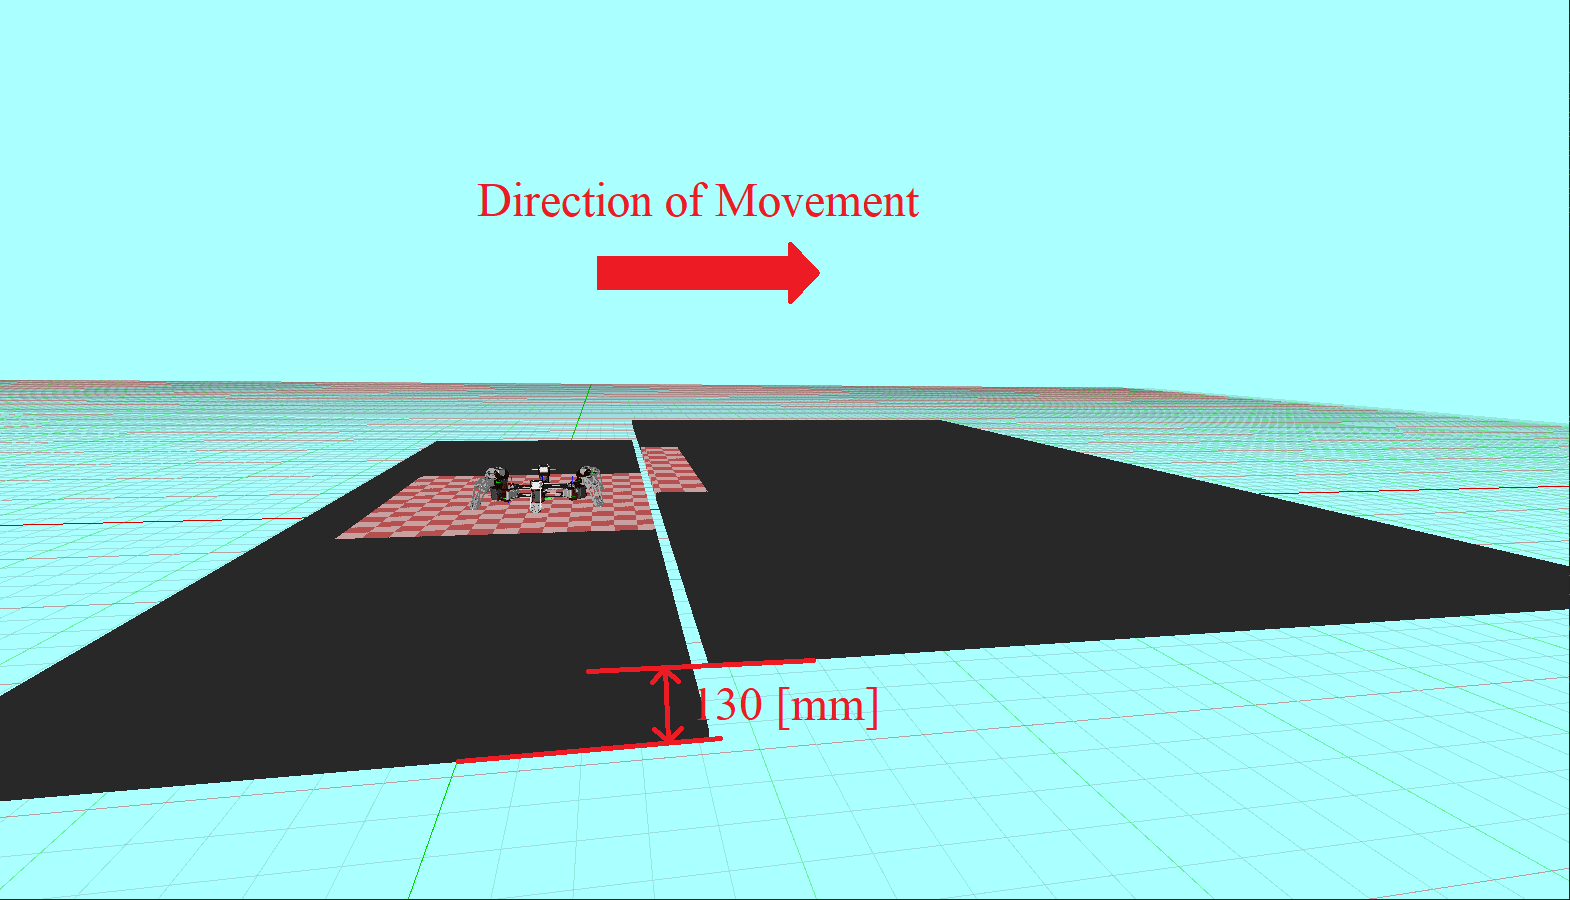
\includegraphics[width=1.0\linewidth]{figure/chapter4/map_130mm.png}
      \text{(b) up step}
      \label{fig:ch5_simu_terrain_up_step} % chktex 24
      \end{center}  
    \end{minipage}
    \\
    &\\  % 空白を入れる
    \begin{minipage}[t]{0.45\hsize}
      \centering
      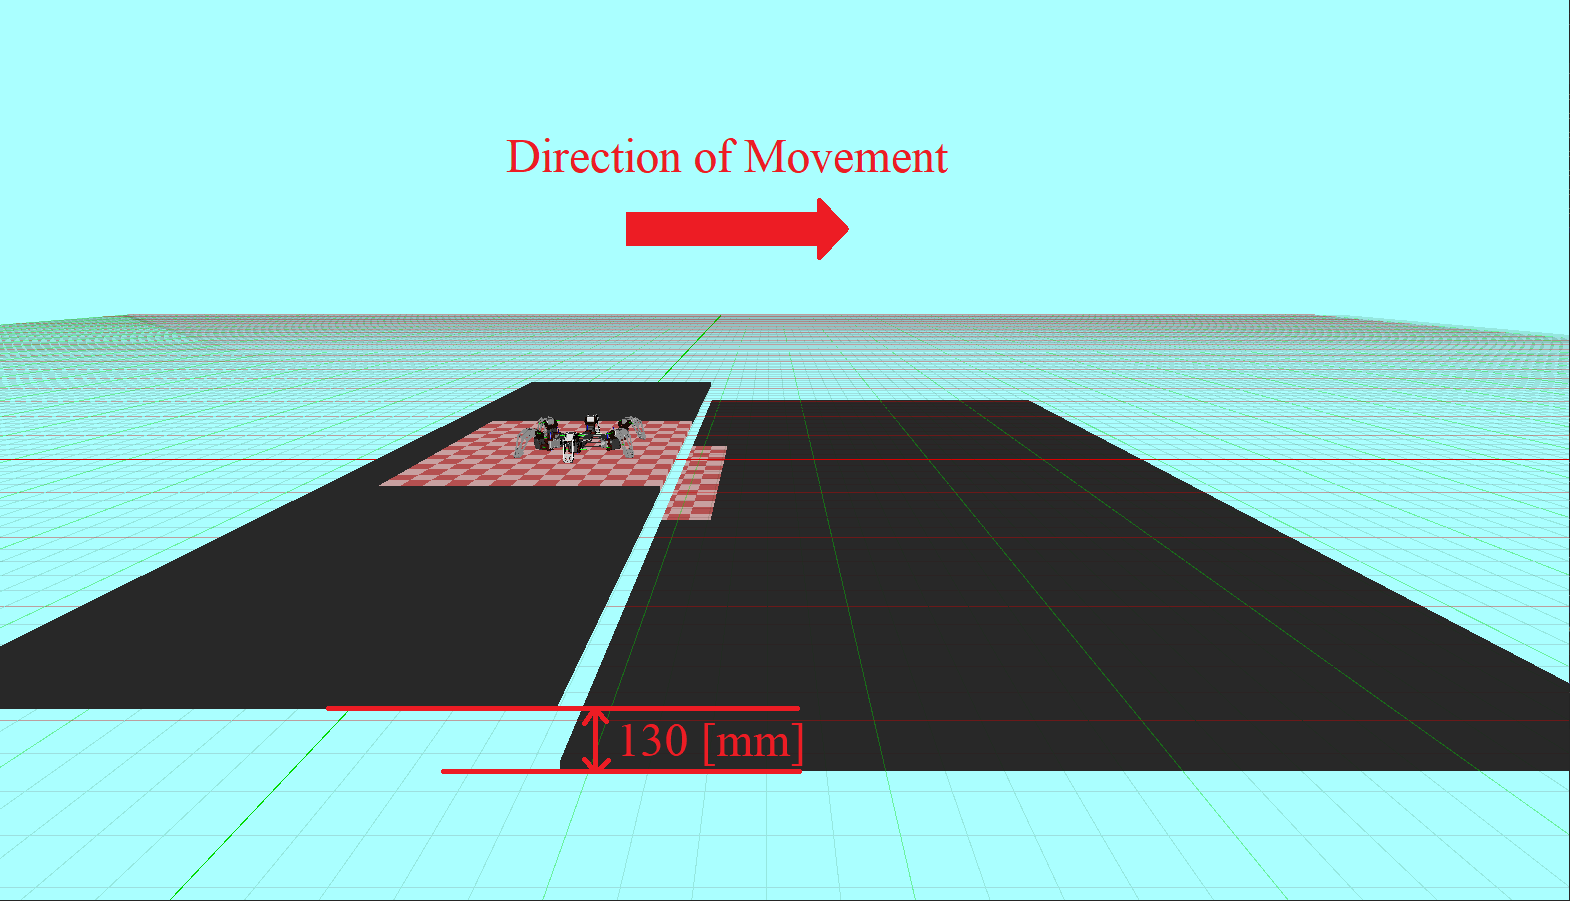
\includegraphics[width=1.0\linewidth]{figure/chapter4/map_-130mm.png}
      \centering
      \text{(c) down step}
      \label{fig:ch5_simu_terrain_down_step} % chktex 24
    \end{minipage} 
    &
    \begin{minipage}[t]{0.45\hsize}
      \centering
      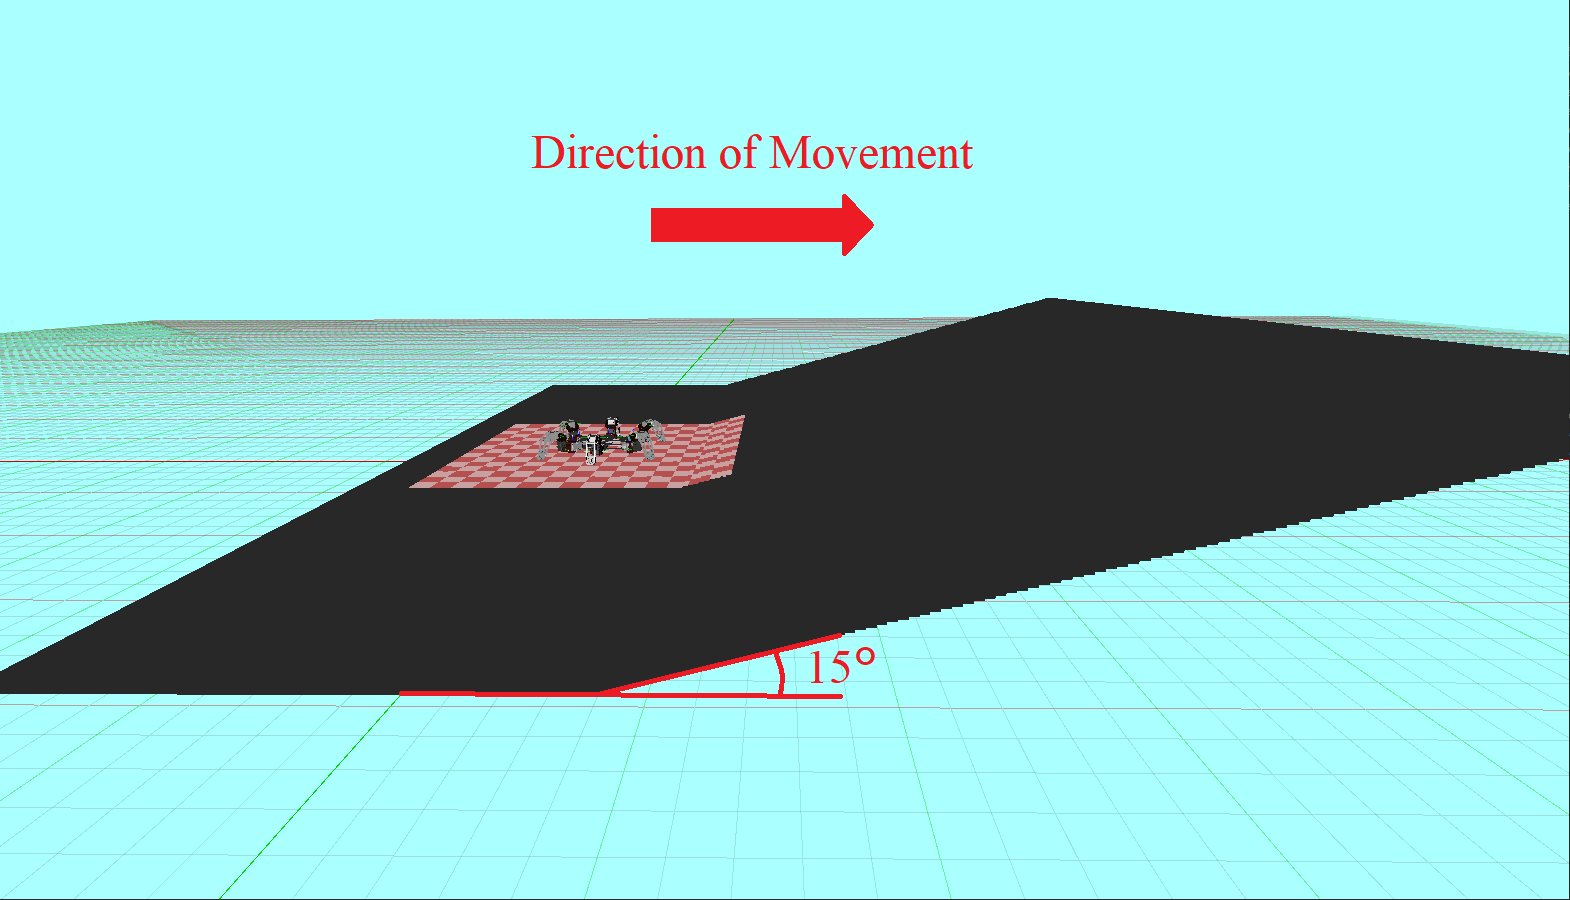
\includegraphics[width=1.0\linewidth]{figure/chapter4/map_15deg.png}
      \centering
      \text{(d) up slope}
      \label{fig:up_slope_terrain} % chktex 24
    \end{minipage}    
    \\
    &\\  % 空白を入れる
    \begin{minipage}[t]{0.45\hsize}
      \centering
      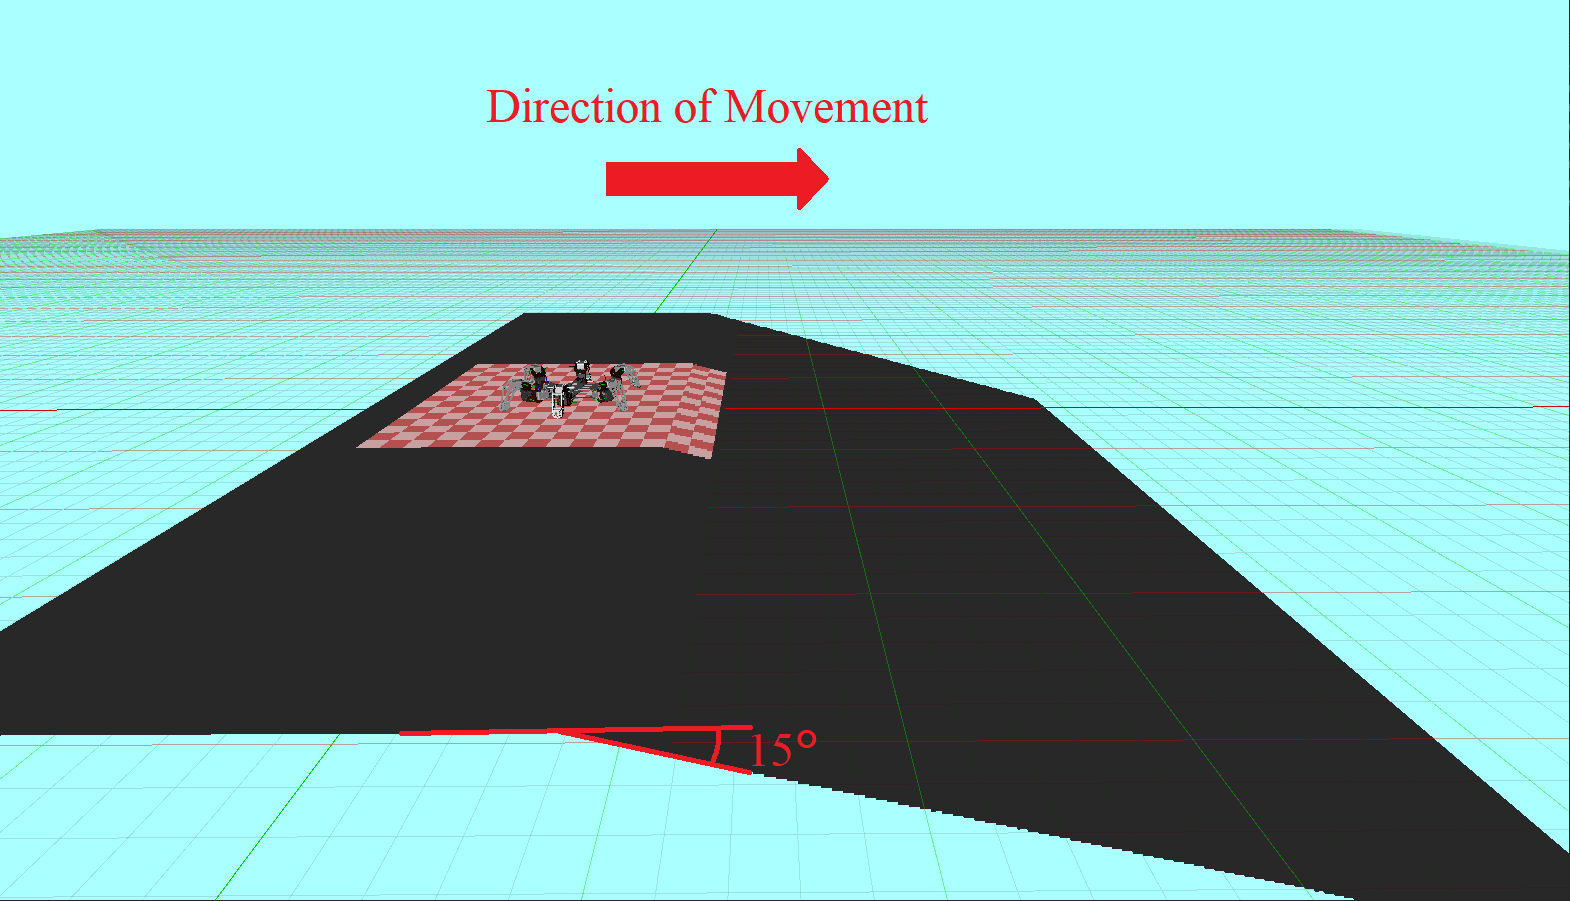
\includegraphics[width=1.0\linewidth]{figure/chapter4/map_-15deg.png}
      \centering
      \text{(e) down slope}
      \label{fig:down_slope_terrain} % chktex 24
    \end{minipage}     
    &
    \\
  \end{tabular}
  \caption{Terrain}
  \label{fig:ch5_simu_terrain} % chktex 24
\end{figure}

\newpage

\subsection{シミュレーション実験の結果}
\subsubsection{脚軌道生成の失敗の回数}
再評価手法を用いた場合の脚軌道生成の失敗の回数を\tableref{tab:ch5_failure_count_1}に示す.
また,再評価手法を用いない場合の脚軌道生成の失敗の回数を\tableref{tab:ch5_failure_count_2}に示す.
この結果から,再評価手法を用いた場合でも,脚軌道生成の失敗が生じてしまうことがわかる.
失敗する場合は,遊脚時に脚軌道が可動範囲外を通ることがわかる.
加えて,初めから最小半径を140mmとすれば,脚軌道生成の失敗は生じていないことがわかる.

\subsubsection{脚先座標}
再評価手法を用いた場合の,脚先座標を地形ごとに\figref{fig:ch5_simu_res_1}に示した.
各図は\figref{fig:ch5_range_revaluation}の$50<x<250,-200<z<0$の範囲を拡大したものである.
脚先座標は支持脚時を青い丸点,遊脚時を赤い丸点で示している.
また,脚軌道生成に失敗した際の脚軌道の中継点を水色の$\times$で示している.
同様に再評価手法を用いない場合の脚先座標を\figref{fig:ch5_simu_res_2}に示した.

これらの結果から,再評価手法を用いた場合でも脚軌道が,
$130 < x < 140$,$-30 < z < -20$の脚の可動範囲外となる領域を通ることがわかる.
また,最初から最小半径を$140 [mm]$とした場合は,脚軌道が可動範囲外を通ることはないことがわかる.

\subsubsection{計算時間}
再評価手法を用いた場合の1つの動作生成にかかる計算時間を\tableref{tab:ch5_calc_time_revaluation}に示す.
また,再評価手法を用いない場合の計算時間を\tableref{tab:ch5_calc_time_140mm}に示す.
これらの表では地形ごとに,計算時間の最大値,最小値,平均,標準偏差を示しており,単位はミリ秒である.

結果より,再評価手法を用いた場合の計算時間の最大値は,用いていない場合の最大値の倍程度となっていることがわかる.
また,再評価手法を用いた場合の計算時間の平均は,用いていない場合と比べて150msec程度大きくなっていることがわかる.

\newpage

\begin{table}[htbp]
  \caption{Failure Count of Revaluation}
  \label{tab:ch5_failure_count_1}  % chktex 24
  \small
  \centering
  \begin{tabular}{|c|c|c|c|c|c|c|c|} \hline  % chktex 44
    \multirow{3}{*}{地形} & \multirow{3}{*}{グラフ探索} & \multicolumn{5}{c|}{失敗の回数} & \multirow{3}{*}{失敗率 $[\%]$} \\ \cline{3-7}  % chktex 44
     & & \multirow{2}{*}{脚接地点が} & \multicolumn{3}{c|}{脚軌道が可動範囲外を通る} & \multirow{2}{*}{総失敗} & \\ \cline{4-6}  % chktex 44
     & の回数 & 可動範囲外 & 遊脚時 & 接地時 & \begin{tabular}{c}胴体平行\\移動時\end{tabular} & 回数 & \\ \hline  % chktex 44
    平面     & 340 & 0 & 21 & 0 & 0 & 0 & 6.17 \\ \hline  % chktex 44
    上り斜面 & 700 & 0 & 35 & 0 & 0 & 0 & 5.00 \\ \hline  % chktex 44
    下り斜面 & 712 & 0 & 18 & 0 & 0 & 0 & 2.52 \\ \hline  % chktex 44
    上り段差 & 500 & 0 & 21 & 0 & 0 & 0 & 4.20 \\ \hline  % chktex 44
    下り段差 & 640 & 0 & 34 & 0 & 0 & 0 & 5.31 \\ \hline  % chktex 44
  \end{tabular}
\end{table}

\begin{table}[htbp]
  \caption{Failure Counts without Revaluation}
  \label{tab:ch5_failure_count_2}  % chktex 24
  \small
  \centering
  \begin{tabular}{|c|c|c|c|c|c|c|c|} \hline  % chktex 44
    \multirow{3}{*}{地形} & \multirow{3}{*}{グラフ探索} & \multicolumn{5}{c|}{失敗の回数} & \multirow{3}{*}{失敗率 $[\%]$} \\ \cline{3-7}  % chktex 44
     & & \multirow{2}{*}{脚接地点が} & \multicolumn{3}{c|}{脚軌道が可動範囲外を通る} & \multirow{2}{*}{総失敗} & \\ \cline{4-6}  % chktex 44
     & の回数 & 可動範囲外 & 遊脚時 & 接地時 & \begin{tabular}{c}胴体平行\\移動時\end{tabular} & 回数 & \\ \hline  % chktex 44
    平面     & 389 & 0 & 0 & 0 & 0 & 0 & 0 \\ \hline  % chktex 44
    上り斜面 & 517 & 0 & 0 & 0 & 0 & 0 & 0 \\ \hline  % chktex 44
    下り斜面 & 689 & 0 & 0 & 0 & 0 & 0 & 0 \\ \hline  % chktex 44
    上り段差 & 513 & 0 & 0 & 0 & 0 & 0 & 0 \\ \hline  % chktex 44
    下り段差 & 681 & 0 & 0 & 0 & 0 & 0 & 0 \\ \hline  % chktex 44
  \end{tabular}
\end{table}


\begin{figure}[htbp]
  \begin{tabular}{cc}
    \begin{minipage}[t]{0.41\hsize}
      \begin{center}
      \includegraphics[width=1.0\linewidth,trim={30 30 30 30}, clip]{figure/chapter4/revaluation/flat.png}
      \text{(a) flat terrain}
      \end{center}
    \end{minipage} 
    &
    \begin{minipage}[t]{0.41\hsize}
      \begin{center}
      \includegraphics[width=1.0\linewidth,trim={30 30 30 30}, clip]{figure/chapter4/revaluation/130mm.png}
      \text{(b) up step terrain}
      \end{center}  
    \end{minipage}
    \\
    \begin{minipage}[t]{0.41\hsize}
      \centering
      \includegraphics[width=1.0\linewidth,trim={30 30 30 30}, clip]{figure/chapter4/revaluation/-130mm.png}
      \centering
      \text{(c) down step terrain}
    \end{minipage} 
    &
    \begin{minipage}[t]{0.41\hsize}
      \centering
      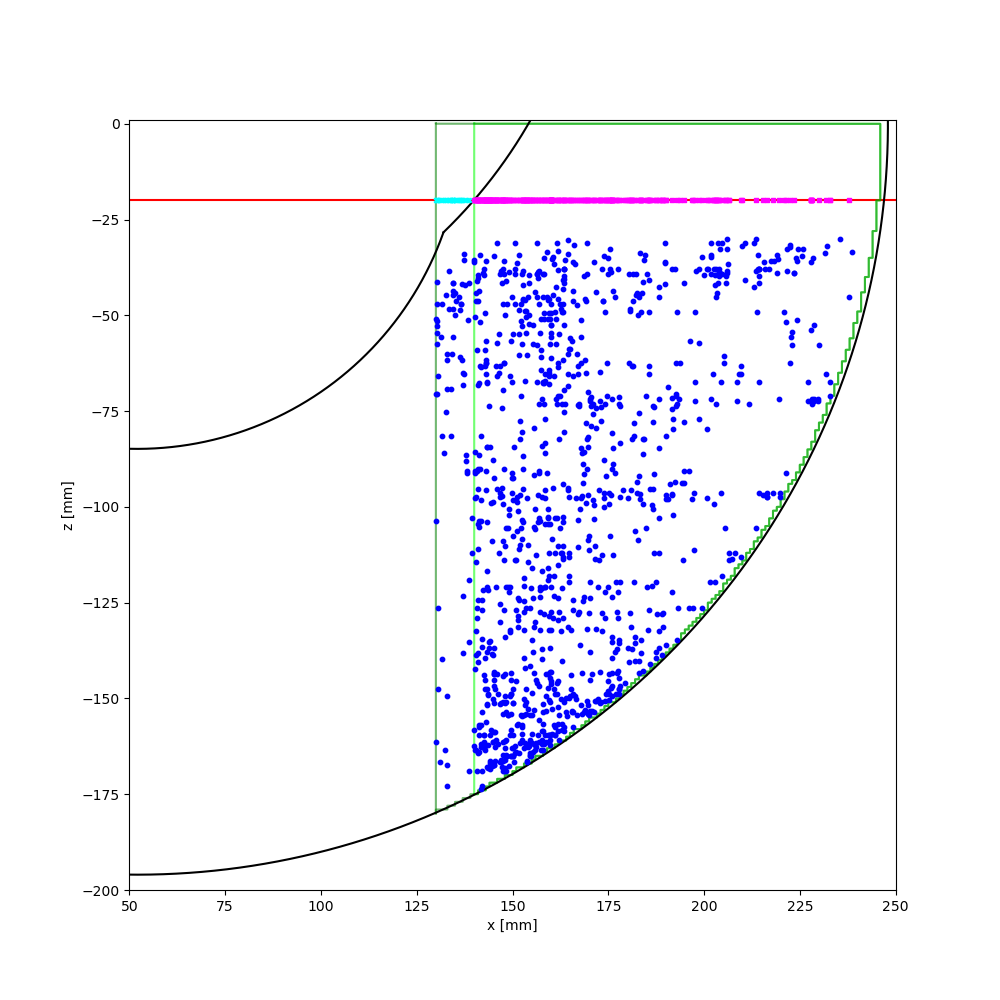
\includegraphics[width=1.0\linewidth,trim={30 30 30 30}, clip]{figure/chapter4/revaluation/15deg.png}
      \centering
      \text{(d) up slope terrain}
    \end{minipage}    
    \\
    \begin{minipage}[t]{0.41\hsize}
      \centering
      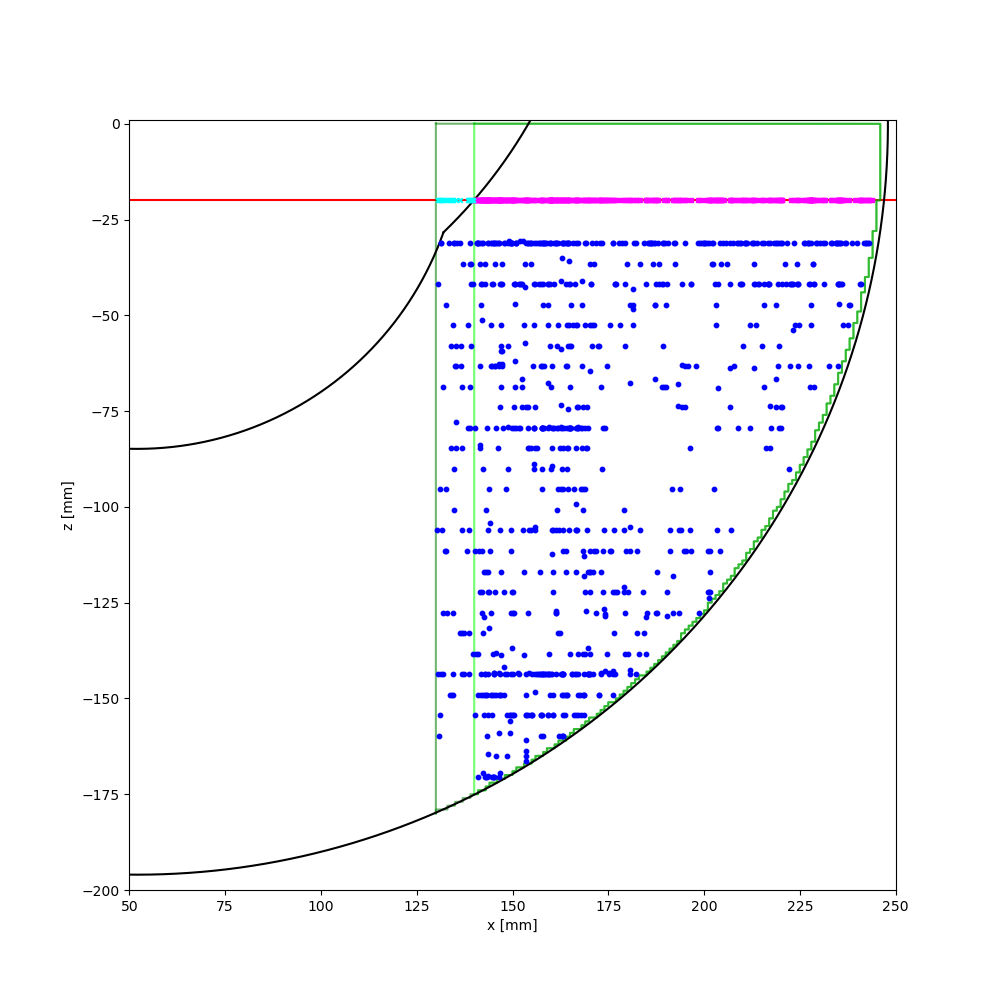
\includegraphics[width=1.0\linewidth,trim={30 30 30 30}, clip]{figure/chapter4/revaluation/-15deg.png}
      \centering
      \text{(e) down slope terrain}
      
    \end{minipage}     
    &
    \\
  \end{tabular}
  \caption{Leg Ground Points for each Terrain (when Revaluation Method)}
  \label{fig:ch5_simu_res_1} % chktex 24
\end{figure}


\begin{figure}[htbp]
  \begin{tabular}{cc}
    \begin{minipage}[t]{0.41\hsize}
      \begin{center}
      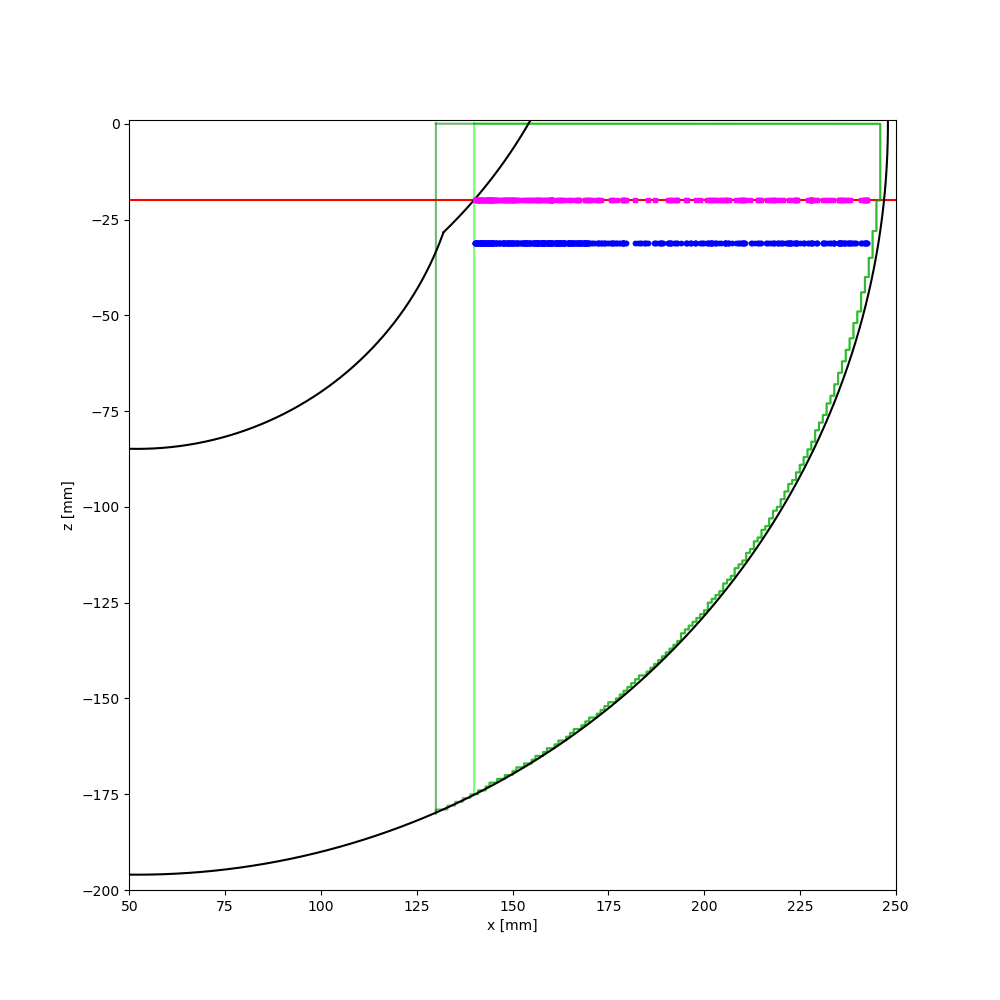
\includegraphics[width=1.0\linewidth,trim={30 30 30 30}, clip]{figure/chapter4/140mm/flat.png}
      \text{(a) flat terrain}
      \end{center}
    \end{minipage} 
    &
    \begin{minipage}[t]{0.41\hsize}
      \begin{center}
      \includegraphics[width=1.0\linewidth,trim={30 30 30 30}, clip]{figure/chapter4/140mm/130mm.png}
      \text{(b) up step terrain}
      \end{center}  
    \end{minipage}
    \\
    \begin{minipage}[t]{0.41\hsize}
      \centering
      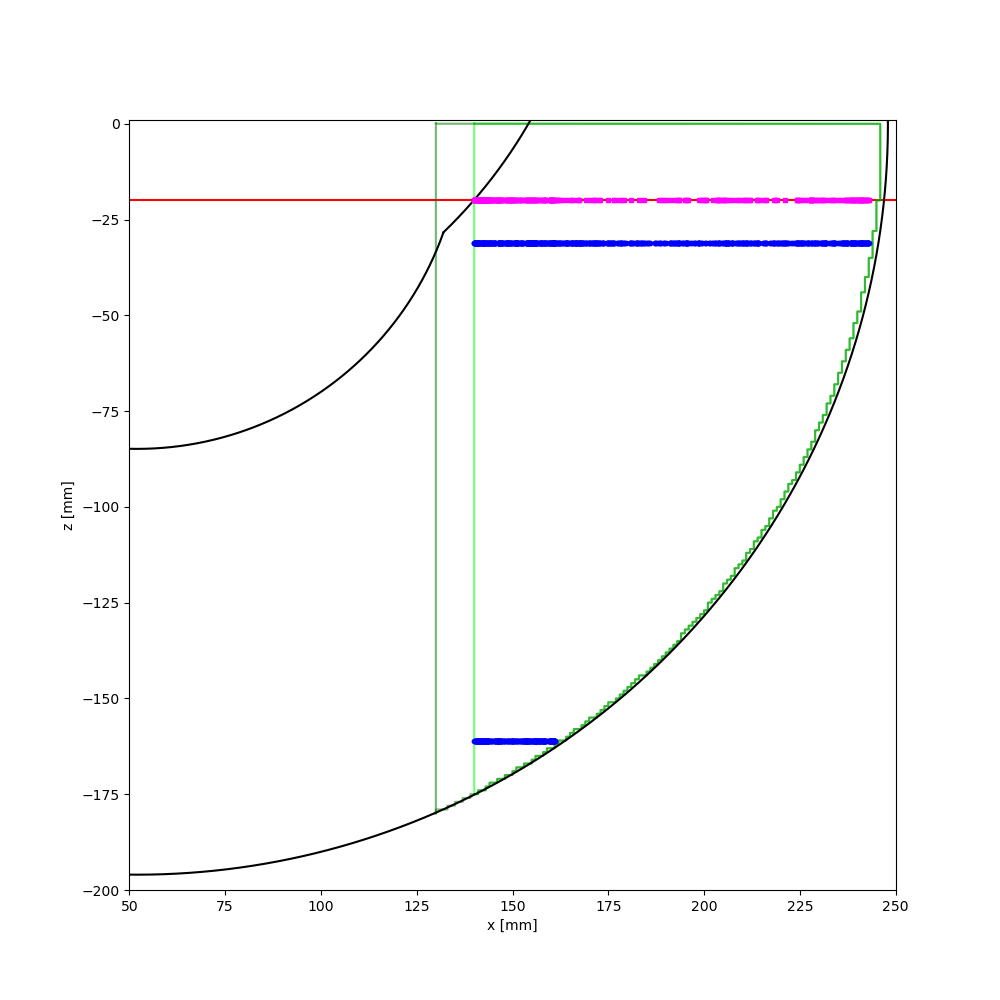
\includegraphics[width=1.0\linewidth,trim={30 30 30 30}, clip]{figure/chapter4/140mm/-130mm.png}
      \centering
      \text{(c) down step terrain}
    \end{minipage} 
    &
    \begin{minipage}[t]{0.41\hsize}
      \centering
      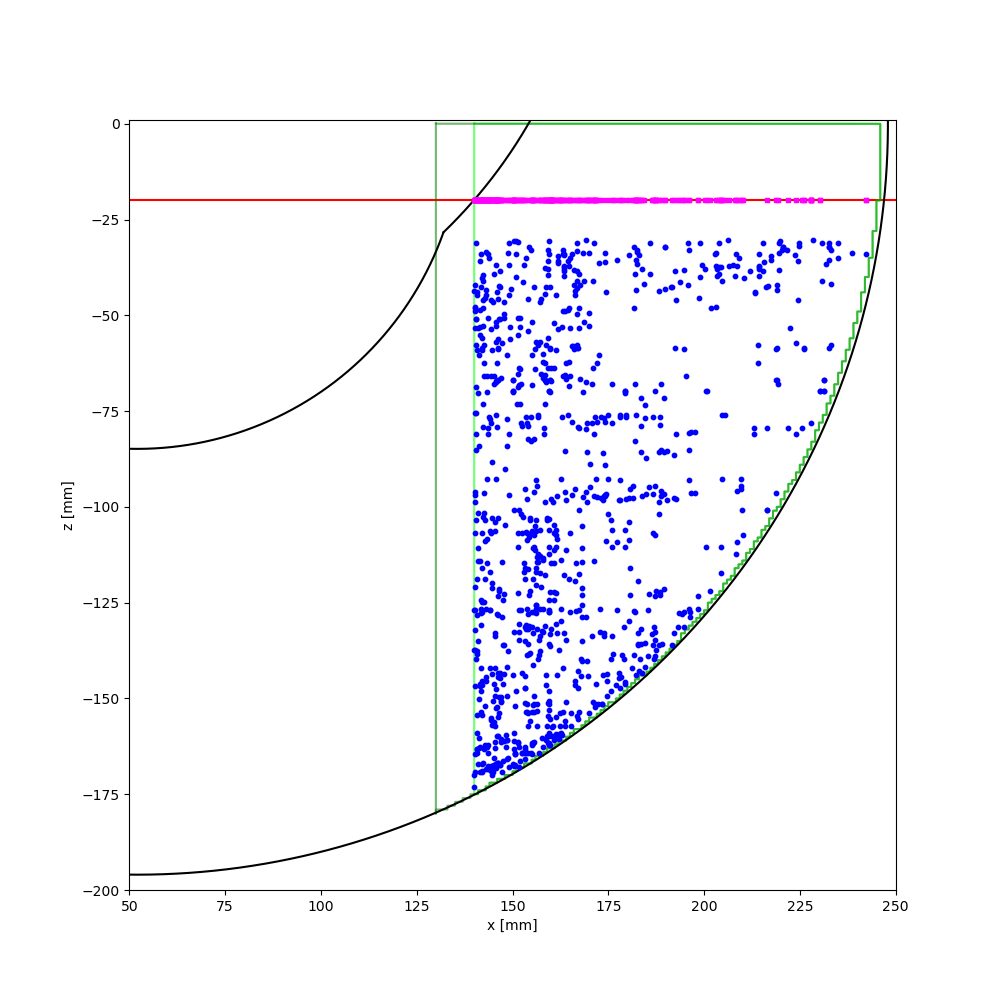
\includegraphics[width=1.0\linewidth,trim={30 30 30 30}, clip]{figure/chapter4/140mm/15deg.png}
      \centering
      \text{(d) up slope terrain}
    \end{minipage}    
    \\
    \begin{minipage}[t]{0.41\hsize}
      \centering
      \includegraphics[width=1.0\linewidth,trim={30 30 30 30}, clip]{figure/chapter4/140mm/-15deg.png}
      \centering
      \text{(e) down slope terrain}
      
    \end{minipage}     
    &
    \\
  \end{tabular}
  \caption{Leg Ground Points for each Terrain (without Revaluation Method)}
  \label{fig:ch5_simu_res_2} % chktex 24
\end{figure}

\newpage


\begin{table}[htbp]
  \caption{Computational Time to Generate One Operation (when Revaluating)}
  \label{tab:ch5_calc_time_revaluation}  % chktex 24
  \centering
  \begin{tabular}{|c||c|c|c|c|} \hline  % chktex 44
    \multirow{2}{*}{地形} & \multicolumn{4}{c|}{1つの動作生成にかかる計算時間} \\ \cline{2-5}  % chktex 44
     & 最大値 $[msec]$ & 最小値 $[msec]$ & 平均 $[msec]$ & 標準偏差 $[msec]$ \\ \hline \hline  % chktex 44
    平面 & 2687 & 14.75 & 655.4 & 606.7 \\ \hline  % chktex 44
    上り段差(130mm)& 2631 & 8.049 & 424.3 & 477.9 \\ \hline  % chktex 44
    下り段差(130mm)& 2761 & 10.53 & 542.7 & 545.3 \\ \hline  % chktex 44
    上り斜面(15度) & 2216 & 14.13 & 436.4 & 409.3 \\ \hline  % chktex 44
    下り斜面(15度) & 4352 & 10.39 & 435.6 & 524.3 \\ \hline  % chktex 44
  \end{tabular}
\end{table}

\begin{table}[htbp]
  \caption{Computational Time to Generate One Operation (without Revaluating)}
  \label{tab:ch5_calc_time_140mm}  % chktex 24
  \centering
  \begin{tabular}{|c||c|c|c|c|} \hline  % chktex 44
    \multirow{2}{*}{地形} & \multicolumn{4}{c|}{1つの動作生成にかかる計算時間} \\ \cline{2-5}  % chktex 44
     & 最大値 $[msec]$ & 最小値 $[msec]$ & 平均 $[msec]$ & 標準偏差 $[msec]$ \\ \hline \hline  % chktex 44
    平面 & 1366 & 16.23 & 463.4 & 351.3 \\ \hline % chktex 44
    上り段差(130mm)& 1364 & 2.975 & 375.9 & 327.2 \\ \hline % chktex 44
    下り段差(130mm)& 1344 & 10.24 & 388.6 & 347.6 \\ \hline % chktex 44
    上り斜面(15度) & 1138 & 4.629 & 271.3 & 263.4 \\ \hline % chktex 44
    下り斜面(15度) & 1286 & 2.364 & 301.9 & 267.0 \\ \hline % chktex 44
  \end{tabular}
\end{table}

\subsection{考察}
再評価手法では歩容パターン生成をやり直す都合上,

結論として,再評価手法によって生成された自由歩容パターンを用いても,脚軌道生成の失敗が生じてしまうことが確認された.
脚の近似された可動範囲における最小半径を140mmとすることで,脚軌道生成の失敗が生じないことを示した.

\section{旋回動作の自由歩容パターン生成シミュレーション}

\section{動作統合時の自由歩容パターン生成シミュレーション}
